\chapter{应用层}\label{CN06}

\par\medskip\noindent\textbf{知识导图}\par\smallskip
\begin{wideblock}\centering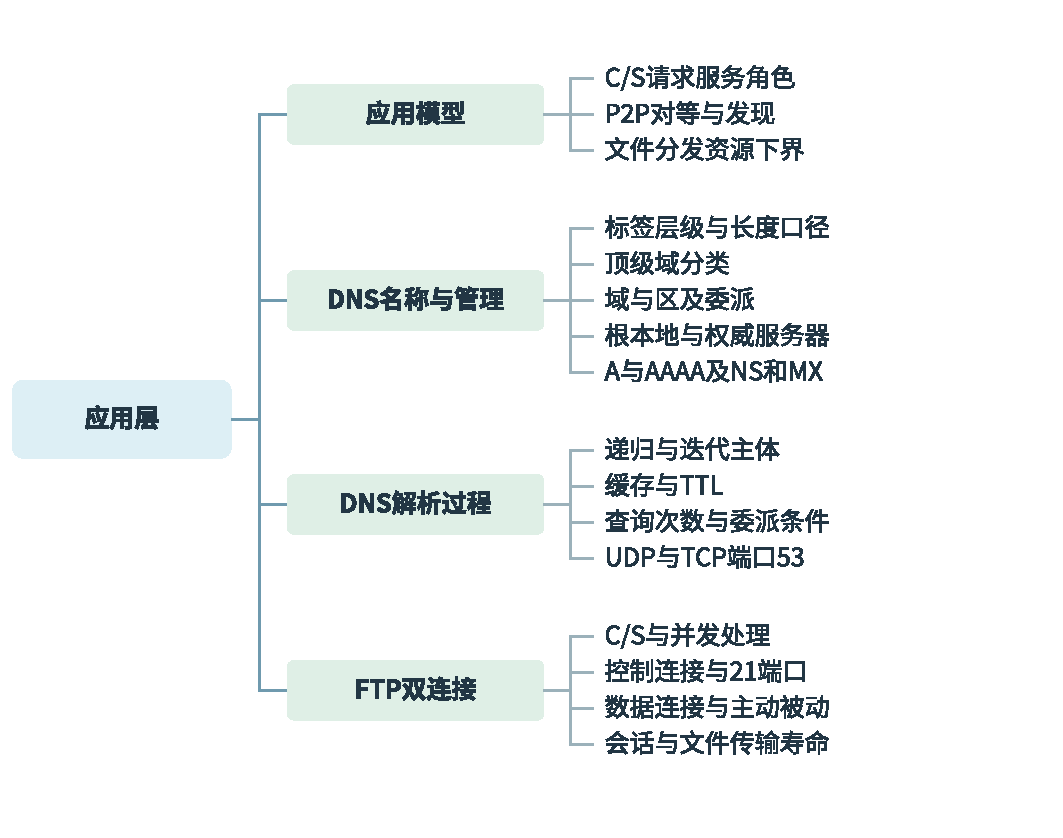
\includegraphics[width=\linewidth,height=168mm,keepaspectratio]{figures/map-01.pdf}\end{wideblock}\par\medskip\clearpage

\par\medskip\noindent\textbf{知识导图（续）}\par\smallskip
\begin{wideblock}\centering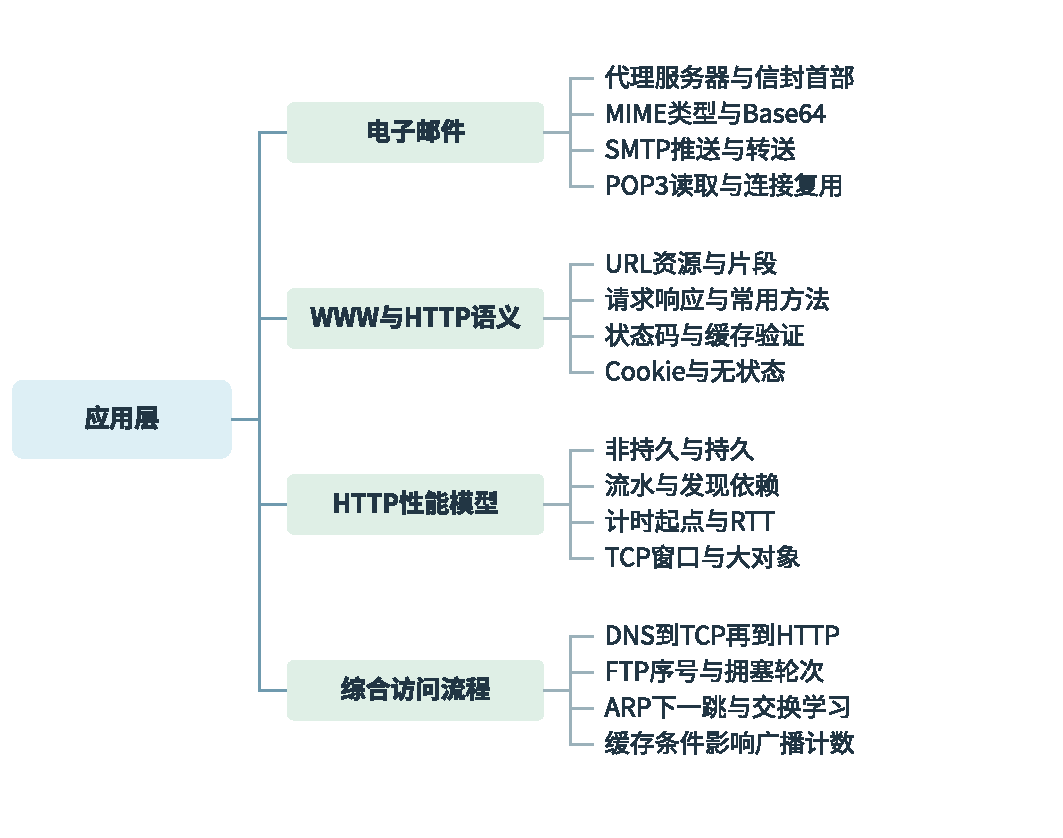
\includegraphics[width=\linewidth,height=168mm,keepaspectratio]{figures/map-02.pdf}\end{wideblock}\par\medskip\clearpage

浏览器中的一个URL同时关联资源名称、服务器地址、传输连接和应用报文。计算访问时间时，要按依赖次序展开：先知道服务器地址，才能连接；先收到并解析HTML，才能知道其中引用哪些资源。缓存命中、连接复用和流水请求改变的是这条依赖链中的具体步骤。

\section{C/S 与 P2P：角色由谁发起服务请求决定}\label{CN06-01}

客户/服务器模型 C/S 中，服务器提供相对稳定的服务入口，客户主动发起请求。服务器可同时服务多个客户，客户不需要一直保持在线。这里``客户''与``服务器''是本次应用交互的角色，不是机器性能等级；同一主机可运行服务器，也可作为其他服务的客户。

P2P让对等节点既能获取资源，也能向其他节点提供资源。它可以减少单一服务器的分发负担，但节点上下线、查找、安全和资源一致性更难管理。P2P应用可以使用集中索引服务器辅助发现节点，不能因为存在一个中心组件，就断言所有数据必须经该中心转发。

以把大小为 \(F\) 的文件分发给 \(N\) 个接收者为例，纯C/S至少要求服务器上传 \(NF\)，因此时间不小于 \(NF/u_s\)；每个接收者还受自身下载速率限制。P2P允许已收到数据的节点继续上传，能增加总上传能力，但仍至少受服务器上传、最慢接收者下载和全系统总上传量等条件限制。这个比较依赖可用上传率和持续参与等条件，不把``P2P更快''写成不受网络约束的绝对结论。

\begin{methodbox}[文件分发先求不可突破的下界]

设服务器上传率\(u_s\)、最慢客户下载率\(d_{\min}\)，客户上传率为\(u_i\)，文件大小为\(F\)，共有\(N\)个客户。纯C/S至少受

\[T_{CS}\ge\max\left(\frac{NF}{u_s},\frac F{d_{\min}}\right)\]

限制；理想P2P还需服务器先贡献至少一份文件，且全系统总上传量要覆盖\(NF\)，因此

\[T_{P2P}\ge\max\left(\frac F{u_s},\frac F{d_{\min}},\frac{NF}{u_s+\sum_i u_i}\right).\]

这些是持续参与、可用速率等理想条件下的必要下界，不能据此保证任意拓扑与实际调度都恰好达到。

\end{methodbox}

推导只需守住数据守恒：纯C/S的\(N\)份副本都由服务器上传；P2P则允许已收到数据的客户继续贡献上传，但所有副本的数据仍必须由系统某处发出。任何一个最慢下载者还必须收到完整\(F\)，因此各资源下界应取最大值，不能相加成三个顺序阶段。

\section{DNS 层次、服务器与区}\label{CN06-02}

DNS把域名与资源记录关联。域名是从右向左逐级具体化的层次名称，完整域名可在末尾带根点。\texttt{www.abc.com}中com为顶级域，abc是其下的一个域，www是进一步的名称标签；不能只按点的个数断言每一级都由独立机器负责。

\begin{definition}[域与权威区]

\textbf{域}是名称空间中的子树，\textbf{区}是由某组权威服务器管理并提供权威数据的范围。一个域可以把某些子域委派出去，因此域与区不必相同。根服务器提供顶级域的委派信息，不存放全世界每台主机的最终地址；权威服务器回答其负责区内的记录。

\end{definition}

常见记录有A（IPv4地址）、AAAA（IPv6地址）、NS（权威服务器）、CNAME（规范名称别名）和MX（邮件交换）。一个名称可以有多个地址，多个名称也可以指向同一个地址，域名、IP与主机之间都不要求一一对应。〖6.2-001〗

域名书写要区分``教材普通主机名规则''与一般DNS记录名称。普通主机名标签常用字母、数字和连字符，大小写不敏感，较低层级写在左侧，顶级域在右侧。单标签最长63字节；DNS线格式完整名称最长255字节，包含标签长度字节和末尾根标签。常见点分文本不带末尾根点时最多253字节，不能把线格式上限不加说明地当成任意显示字符串的字符上限。

顶级域可区分国家/地区类（如cn）、通用类（如com、org）与基础设施用途的arpa等。管理层级与实际服务器部署不是一一对应，反向名称解析的组织也不能简单写成把IP字符串交给普通A记录查询。

本地域名服务器即递归解析器，通常由组织或运营商等提供，位置不必与主机处在同一个以太网内。主机先查浏览器或系统缓存，再向配置的解析器发出请求；不能把本地解析器直接等同于根服务器。

\section{递归、迭代与缓存：谁又发了一次查询}\label{CN06-03}

递归查询要求被请求的服务器继续完成解析，最终返回答案或失败；迭代查询允许服务器返回下一步应询问的服务器信息，由原查询者继续询问。常见流程是主机向本地解析器请求递归服务，本地解析器依次对根、顶级、权威服务器进行迭代查询。

例如解析 \texttt{www.abc.com}：本地解析器先问根，取得com的服务器信息；再问com，取得abc.com的权威服务器；最后问权威服务器取得Web地址。缓存中若已有最终A/AAAA记录，可不发远程查询；若只有某级委派，可以从该级继续。缓存受TTL有效期限制，不能无条件永久使用。

比较递归与迭代时，固定三件事：当前谁提出查询，收到的答复是最终答案还是下一站信息，由谁发下一条查询。递归把继续解析的工作交给被请求者，迭代让当前查询者沿委派继续。缓存命中只会改变需要走几步，并不改变这两种交互的定义；``用了缓存''也不能直接推出请求来自根服务器还是本地解析器。

\subsection{例 6-1　问的是本地服务器发出多少次查询}\label{CN06-ex1}

\begin{example}[配套例题]

配套例题。 假设所有域名服务器均采用迭代查询方式进行域名解析。当H4访问规范域名为 \texttt{www.abc.xyz.com} 的网站时，域名服务器201.1.1.1完成该域名解析过程中，可能发出DNS查询的最少和最多次数分别是（　）。共用网络拓扑如下。

\par\medskip\noindent\begin{minipage}{\linewidth}
\centering
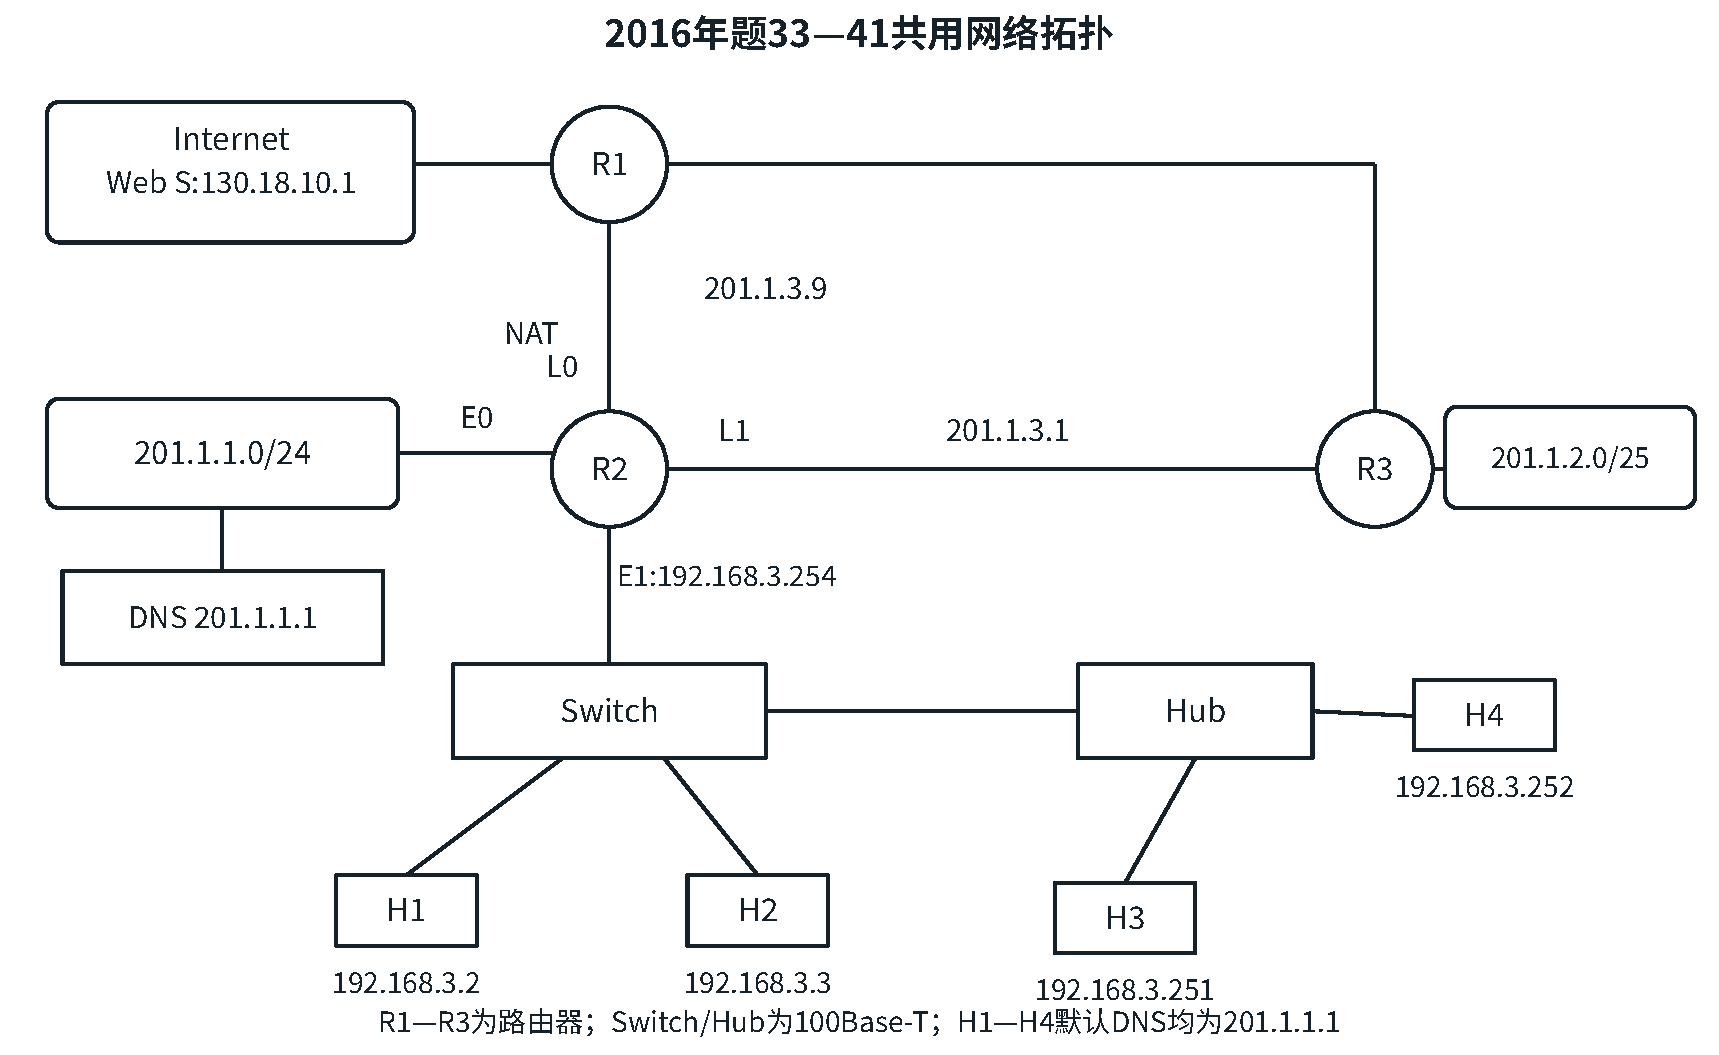
\includegraphics[width=\linewidth,height=125mm,keepaspectratio]{figures/CN14_dns_topology_2016.pdf}
\captionof{figure}{2016年共用拓扑；本题只使用H4及其默认DNS服务器201.1.1.1}\label{cn-fig-dns2016}
\end{minipage}\par\medskip

A. 0，3　B. 1，3　C. 0，4　D. 1，4

\end{example}

\textbf{解析。} 计数主体是201.1.1.1，不是H4。最终地址在有效缓存中时，本地服务器不需向外查询，最少0次；完全无可用缓存，且相应各级分别委派时，可依次询问根、com、xyz.com、abc.xyz.com，共4次，选 \textbf{C}。H4向201.1.1.1的最初请求不是这台服务器``发出''的请求，不能加入。

``最多4次''采用原题的规范域名及逐级委派模型，不计别名链、失败重试或负载均衡额外查询。若改问主机发出几条请求，或所有层级均以递归方式向下转交，通信主体与计数就要重新列出，而不是照抄0、4。

DNS常用UDP端口53，也支持TCP，例如区域传送、较大响应或按协议退回TCP的场景。不能简单断言DNS只用UDP，更不能将``DNS也能用TCP''误读为每次普通查询都必须先三次握手。

\section{FTP：控制命令与文件数据为什么分两条连接}\label{CN06-04}

FTP运行在TCP上，控制连接用于登录、目录、传送命令与状态回复，服务器熟知端口为21；数据连接用于文件或目录数据。在一次会话中，控制连接可持续存在，多次传送按需要建立、关闭数据连接，控制报文因此不必夹在文件字节流里，也能被识别。

\subsection{例 6-2　传递 FTP 命令使用哪条连接}\label{CN06-ex2}

\begin{example}[配套例题]

配套例题。 FTP客户和服务器间传递FTP命令时，使用的连接是（　）。

A. 建立在TCP之上的控制连接

B. 建立在TCP之上的数据连接

C. 建立在UDP之上的控制连接

D. 建立在UDP之上的数据连接

\end{example}

\textbf{解析。} 先由``FTP命令''确定控制连接，再由FTP的传输协议确定TCP，选 \textbf{A}。文件内容放在数据连接；登录服务器时，第一阶段建立的也是控制连接，不能等文件传送结束后才建立命令通道。〖6.3-005〗

主动模式由服务器向客户指定的地址和端口发起数据TCP连接，传统服务器数据源端口为20；被动模式由服务器通告监听端口，再由客户主动连接该数据端口。不能说``所有FTP数据连接的服务器端口永远为20''，也不能把主动/被动模式误解为控制连接的建立顺序。

教材常用``一个监听主进程，加多个会话控制/数据处理任务''解释FTP并发：监听21端口的入口接收新客户，每个会话维护自己的控制状态，具体文件传输再使用数据连接。实际服务器可用进程、线程或事件驱动实现，概念模型不要求每条连接都必须创建一个操作系统进程。

\section{邮件系统、邮件格式与 MIME}\label{CN06-05}

邮件系统包括用户代理、邮件服务器和传送协议。用户代理负责编辑、显示和管理邮件，邮件服务器负责队列、邮箱及服务器间传送。一个``发送成功''的界面提示，可能只表示本机或提交服务器接受了邮件，不等于对方用户已经读取。

邮件由首部和正文组成，以空行分隔；首部中的From、To、Subject等表达用户可见信息，传输过程中SMTP还使用信封发件人与收件人控制实际投递。这两套地址可能不同，不能仅按邮件里显示的地址推断所有投递端点。

基础SMTP按7位ASCII文本传输，不能直接把任意二进制图像当作普通7位正文。MIME定义内容类型、字符集、传送编码和多部分结构，使非ASCII文字与附件能表示为可传送内容。例如Base64将3字节转成4个ASCII字符，载荷大约膨胀到原来的4/3，此外还有格式开销。编码不是加密，收件人仍可按公开规则恢复原内容。现代扩展可协商更丰富的能力，作基础SMTP题时先确认题目采用哪一种范围。

\section{SMTP 负责发送，POP3 负责读取}\label{CN06-06}

SMTP是推送协议，用于用户代理提交邮件、以及邮件服务器之间转送邮件；服务器间常用TCP端口25，用户提交还常见经认证的提交服务。POP3是读取协议，用于用户代理从邮件服务器取邮件，基本服务使用TCP端口110。协议名区分的是应用动作，不能因为都处理邮件就认为两者可以相互代替。

典型路径为：发送者用户代理通过SMTP提交\ensuremath{\to}发送方邮件服务器按队列与DNS中的MX记录寻找收件域邮件服务器\ensuremath{\to}服务器间通过SMTP转送\ensuremath{\to}收件用户代理用POP3等读取。使用Web邮箱时，浏览器与Web服务还可能使用HTTP，后端仍另有邮件传送机制。

POP3依次经过授权、事务处理和更新等阶段。用户可列出、读取多封邮件，删除通常要等到会话的相应更新阶段才落实；不能把``读取''无条件等同于立即从服务器删除，也不能说一封邮件必新建一条TCP连接。

\subsection{例 6-3　一次 POP3 连接可以读几封邮件}\label{CN06-ex3}

\begin{example}[配套例题]

配套例题。 下列关于POP3协议的叙述中，正确的是（　）。

I. 支持用户代理从邮件服务器读取邮件

\begin{enumerate}
\def\labelenumi{\Roman{enumi}.}
\setcounter{enumi}{1}
\item
  支持用户代理向邮件服务器发送邮件
\item
  支持邮件服务器之间发送与接收邮件
\item
  支持通过一条TCP连接收取多封邮件
\end{enumerate}

A. 仅I、IV　B. 仅II、III　C. 仅I、II、III　D. 仅I、III、IV

\end{example}

\textbf{解析。} POP3用于用户代理读取，I正确；发送和服务器间转送由SMTP等机制承担，II、III错误；事务阶段可在同一TCP连接内处理多封邮件，IV正确，选 \textbf{A}。决定答案的是协议负责哪个方向，而不是``都传邮件''这个共同点。

\section{WWW、URL 与资源位置}\label{CN06-07}

WWW用超链接把资源组织起来，浏览器按URL定位和访问资源。URL常包含方案、主机、可选端口、路径、查询及片段。例如 \texttt{http:\allowbreak{}/\allowbreak{}/\allowbreak{}www.abc.com:\allowbreak{}80/\allowbreak{}index.html?q=\allowbreak{}408\#part1} 中，http决定访问方案，主机名用于解析服务器地址，路径和查询参与HTTP请求定位，\texttt{\#part1}由浏览器用于文档内定位，不作为普通HTTP请求目标发送给服务器。

网页不是必然只有一份文件。HTML可再引用图片、脚本、样式表等对象，浏览器通常要先收到HTML，或在解析过程中逐步发现这些地址。它们可能来自同一服务器，也可能来自不同域名，需要另作DNS或连接判断。不能把``同一个页面''当成``只需要一个网络往返''。

HTTP是应用层协议，通常运行在TCP上；HTTPS在HTTP通信中加入TLS等安全机制。本章时延题采用题目明确的HTTP/1.0或HTTP/1.1模型，不把HTTP/2多路复用或HTTP/3的QUIC机制混入旧题。高版本存在，不会自动修改题干所限定的协议行为。

\section{HTTP 请求、连接复用、缓存与时延}\label{CN06-08}

HTTP请求行包含方法、请求目标、版本，后接首部、空行和可选消息体；响应包含状态行、首部及消息体。GET常用于获取资源，HEAD获取对应首部信息，POST提交数据；方法名本身并不决定服务器是否改变状态，还要看协议语义和实际处理。状态码200表示请求成功，301/302表示重定向，304用于条件请求中的资源未改动，404表示未找到等。

HTTP被称为无状态协议，是指一次请求的处理不自动要求服务器记住上次会话状态。Cookie可以让客户随请求携带标识，服务器据此关联状态；持久TCP连接则减少反复建立连接的开销。\textbf{无状态、Cookie和连接是否持久是三个不同问题}，不能相互推出。

非持久HTTP通常每个对象使用一条TCP连接，题目忽略发送时延，一个小对象至少需要1RTT建立连接、1RTT完成请求响应。若允许多个连接并行，可在发现对象后并行获取；若不允许并行，各对象就串行承担这两项。持久HTTP在同一连接上取多个对象，非流水方式仍按请求响应逐个等待；HTTP/1.1流水线允许前一响应尚未完成就发后续请求，但尚不知道的资源地址无法凭空提前请求。

只有条件一致，比较才有可计算的结果：DNS已完成、TCP尚未建立，HTML引用同站的 \(m\ge1\) 个小对象，必须先收到HTML才知道它们；不并行建连接，忽略报文传输、处理、拥塞与流量控制，所有往返均为同一个RTT。

\begin{wideblock}

\par\medskip\noindent\begin{minipage}{\linewidth}\fontsize{9.3}{12}\selectfont\begin{tabularx}{\linewidth}{@{}YYYY@{}}
\toprule\noalign{}
\begin{minipage}[b]{\linewidth}\raggedright
模型
\end{minipage} & \begin{minipage}[b]{\linewidth}\raggedright
TCP连接复用
\end{minipage} & \begin{minipage}[b]{\linewidth}\raggedright
对象请求能否重叠
\end{minipage} & \begin{minipage}[b]{\linewidth}\raggedright
从建立首连接到收齐的时间
\end{minipage} \\
\midrule\noalign{}


非持久、串行 & 每个对象另建，共 \(m+1\) 条 & 每次取完再建立下一条 & \(2(m+1)RTT\) \\
持久、非流水 & 所有对象共用一条 & HTML及后续对象逐个等待 & \((m+2)RTT\) \\
持久、流水 & 所有对象共用一条 & HTML后，已知的 \(m\) 个请求可连续发出 & \(3RTT\) \\
\bottomrule\end{tabularx}
\end{minipage}\par\medskip

\end{wideblock}

三行都包含首次TCP建立的1RTT；若计时从已建连接上的HTTP请求发出开始，应各自去掉这一项。流水的3RTT仍含``握手---HTML---后续对象''三个依赖阶段；若对象较大、窗口不足或来自不同服务器，这张表的理想时间就不再直接适用。下面例题只改变其中的起点、并行条件或窗口约束。

\begin{methodbox}[HTTP时延按依赖分段]

先核对DNS是否完成、TCP是否已建，再问HTML何时揭示资源地址；在后续资源阶段才区分是否并行、是否复用、是否流水。之后叠加题目明确给出的发送、拥塞窗口和处理开销。每次减少一个RTT，都应说明是哪次握手或等待被免去。

\end{methodbox}

\begin{example}[请求目标不包含片段标识]

访问\texttt{http:\allowbreak{}/\allowbreak{}/\allowbreak{}www.abc.com/\allowbreak{}index.html?q=\allowbreak{}408\#part1}，在题设HTTP/1.1模型中，请求可写为：

\begin{codeblock}[language={}]
GET /index.html?q=408 HTTP/1.1
Host: www.abc.com
\end{codeblock}

\end{example}

路径与查询串交给服务器定位资源，\texttt{\#part1}留给浏览器在文档内定位；这段请求文本并未把DNS、TCP握手或TLS开销包含进去，计时仍须按题设另算。

\subsection{例 6-4　非持久且不允许并行，要算上 HTML 本身}\label{CN06-ex4}

\begin{example}[配套例题]

配套例题。 若浏览器不支持并行TCP连接，使用非持久的HTTP/1.0协议请求浏览1个Web页，该页中引用同一网站上的7个小图像文件，则从浏览器为传输Web页请求建立TCP连接开始，到接收完所有内容为止，所需要的RTT数至少是（　）。

A. 4　B. 9　C. 14　D. 16

\end{example}

\textbf{解析。} 一共8个对象：HTML与7张图片。每个对象单独建立TCP连接并请求响应，各2RTT，且题目禁止并行，故总计 \(8\times2=16RTT\)，选 \textbf{D}。只计算7张图会得到14，遗漏页面本身。题干计时从请求建立连接开始，不是从HTTP请求已经发出后开始。

\subsection{例 6-5　流水线仍不能跨过资源发现依赖}\label{CN06-ex5}

\begin{example}[配套例题]

〖6.5-012〗 假设主机通过HTTP/1.1流水线方式请求Web服务器上的rfc.html，它引用同目录下3个JPEG小图像，只有收到rfc.html后才能发送对应图像请求。一次请求响应为RTT，忽略其他时延，不考虑拥塞与流量控制。从发出HTTP请求报文开始，到收到全部内容，所耗时间是（　）。

A. 2RTT　B. 2.5RTT　C. 4RTT　D. 4.5RTT

\end{example}

\textbf{解析。} 起点已经是HTTP请求发出，不再加TCP握手。第1RTT取HTML，得到3个图片地址；3个请求可流水发送，忽略传输时延时，再1RTT收到图片，共2RTT，选 \textbf{A}。若题目不允许流水，应在同一连接逐对象等待，HTML及3图共4RTT。只有改变请求能否重叠这类条件，计算才会改变；不能把``持久''一词直接等同于1RTT。

\par\medskip\noindent\begin{minipage}{\linewidth}
\centering
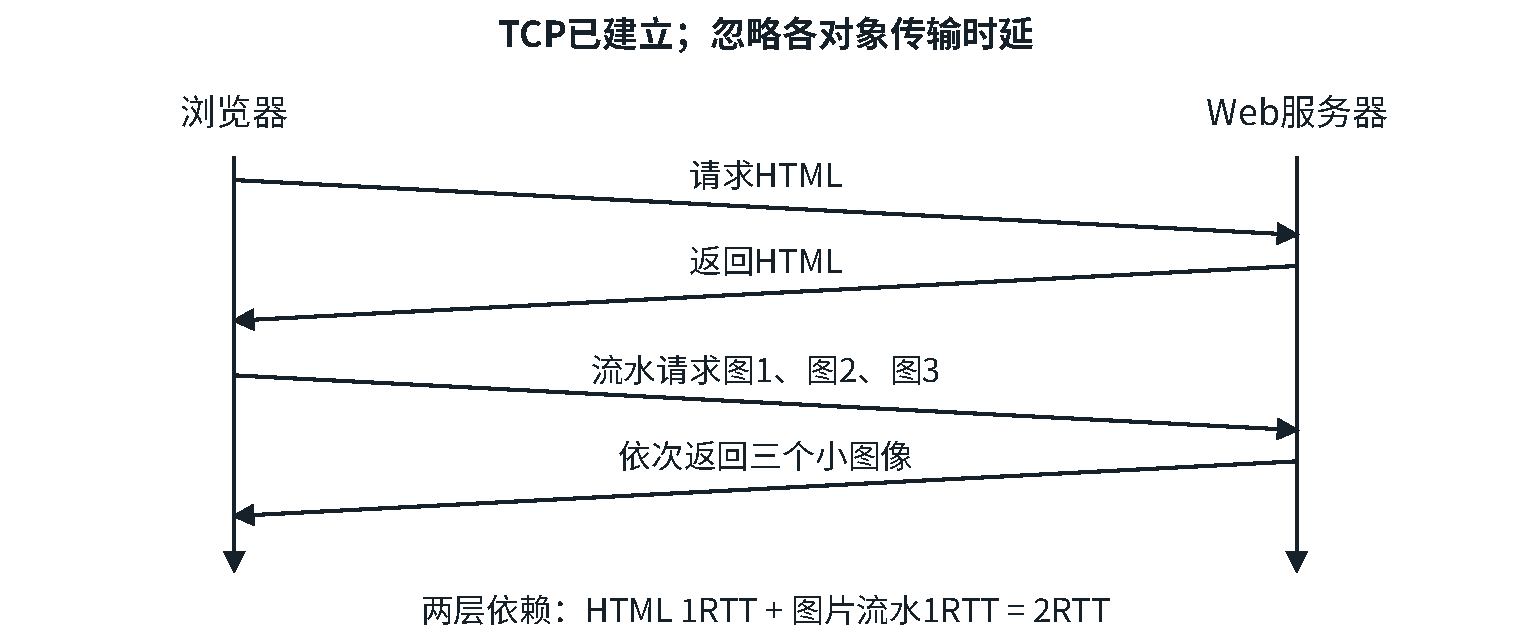
\includegraphics[width=\linewidth,height=125mm,keepaspectratio]{figures/CN12_http_pipeline.pdf}
\captionof{figure}{连接已建立时，HTML完成后才能发送三个图片请求；流水阶段可重叠}\label{cn-fig-http}
\end{minipage}\par\medskip

\subsection{例 6-6　DNS 与 Web 的时间由哪几项组成}\label{CN06-ex6}

\begin{example}[配套例题]

配套例题。 假设下图网络中的本地域名服务器只提供递归查询服务，其他域名服务器均只提供迭代查询服务；局域网内主机访问Internet上各服务器的RTT均为10 ms，忽略其他各种时延。若主机H通过超链接 \texttt{http:\allowbreak{}/\allowbreak{}/\allowbreak{}www.abc.com/\allowbreak{}index.html} 请求浏览纯文本Web页index.html，从单击超链接到浏览器收到页面，所需的最短与最长时间分别是（　）。

\par\medskip\noindent\begin{minipage}{\linewidth}
\centering
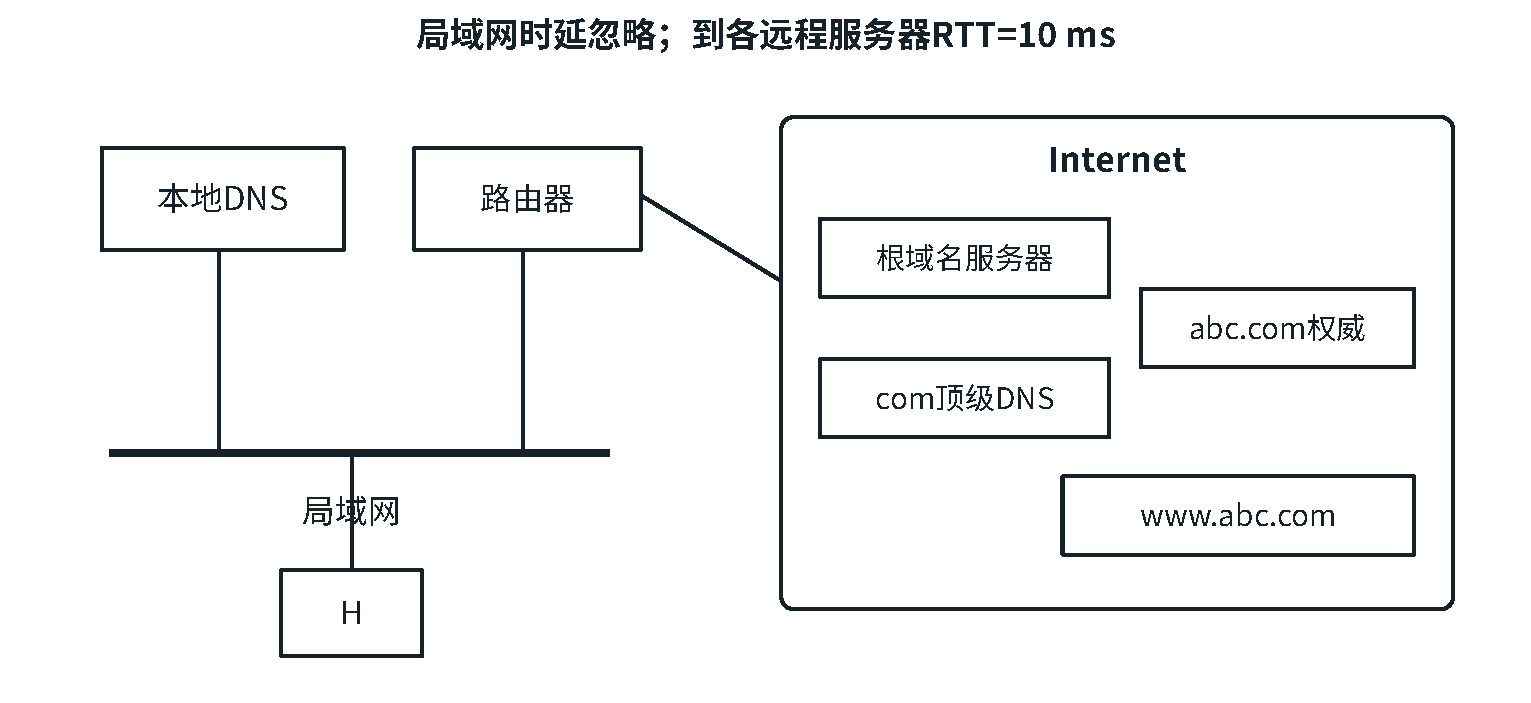
\includegraphics[width=\linewidth,height=125mm,keepaspectratio]{figures/CN11_dns_web_2020.pdf}
\captionof{figure}{主机、本地DNS与路由器共享局域网，远程服务器分别承担名称解析和Web响应}\label{cn-fig-dns2020}
\end{minipage}\par\medskip

A. 10 ms，40 ms　B. 10 ms，50 ms

C. 20 ms，40 ms　D. 20 ms，50 ms

\end{example}

\textbf{解析。} 采用题目首次取页面、尚未建立目标TCP连接的模型。有效DNS缓存命中时，不需要远程DNS往返，但TCP建立与HTTP请求响应各1RTT，最短20 ms。完全无所需缓存时，本地解析器依次询问根、com、abc.com权威服务器，增加3RTT；再取Web共5RTT=50 ms，选 \textbf{D}。主机与本地DNS之间的局域网时延已忽略，不能额外加一次10 ms。

如果题目再允许浏览器已缓存新鲜的HTML副本，可能无须访问服务器；若TCP已经建立，也会少一个握手往返。这些是改变原题模型的附加条件，不能在原题中任意引入后声称存在另一个更短答案。

\subsection{例 6-7　收到 HTML 后，拥塞窗口还限制图片分几轮}\label{CN06-ex7}

\begin{example}[配套例题]

配套例题。 假设主机H通过HTTP/1.1请求Web服务器S上的news408.html，它引用同目录下1幅图像。HTML文件大小为1 MSS，图像3 MSS，RTT=10 ms，忽略HTTP响应首部开销和TCP段传输时延。若H已完成域名解析，则从H请求与S建立TCP连接时刻起，到收到全部内容，所需的时间至少是（　）。

A. 30 ms　B. 40 ms　C. 50 ms　D. 60 ms

\end{example}

\textbf{解析。} 原题答案采用教材模型：慢开始初始窗口为1 MSS，使用同一条持久连接，HTML收到后才请求图像。TCP建立用1RTT；HTML请求与1 MSS响应再1RTT，服务器收到其确认后窗口可增长为2 MSS；图像有3 MSS，先发2 MSS，收到确认后再发余下1 MSS，图片阶段还需2RTT。因此共4RTT=40 ms，选 \textbf{B}。

这里题源未在题干单独写初始拥塞窗口，不能把结论推广为所有HTTP/1.1实现的固定最短时间。若明确允许较大初始拥塞窗口，3 MSS图片可在一轮内返回，则题目的数值会改变。遇到这类题，应在计算旁写清采用的TCP初态，不能一边沿用1 MSS答案、一边声称初态完全无关。

HTTP缓存还要区分新鲜命中和条件验证。新鲜缓存可直接响应而不向源站发送请求；过期或需重新验证时，可用If-Modified-Since或If-None-Match等条件请求，服务器返回304时不传原完整实体，但验证过程仍有请求响应时延。代理缓存能缩短远程路径、减少上游流量，但并不意味着缓存中的对象永不改变。

回看各应用协议，可按``谁向谁做什么、用何种传输、端口属于哪一方''比较，不能只把名称和端口罗列成表，就以为各协议可以互相替代。

\begin{wideblock}

\par\medskip\noindent\begin{minipage}{\linewidth}\fontsize{9.3}{12}\selectfont\begin{tabularx}{\linewidth}{@{}YYYY@{}}
\toprule\noalign{}
\begin{minipage}[b]{\linewidth}\raggedright
应用任务与协议
\end{minipage} & \begin{minipage}[b]{\linewidth}\raggedright
主要交互端点和动作
\end{minipage} & \begin{minipage}[b]{\linewidth}\raggedright
本章基本承载与端口
\end{minipage} & \begin{minipage}[b]{\linewidth}\raggedright
需要保留的条件
\end{minipage} \\
\midrule\noalign{}


名称解析DNS & 主机/解析器向DNS服务器询问记录 & UDP或TCP，服务端53 & 缓存、递归/迭代决定查询路径；不是每次必经根 \\
自动配置DHCP & 客户向服务器申请地址与其他配置 & UDP，服务器67、客户68 & 初始广播与续租单播要按阶段判断 \\
文件传送FTP & 客户和服务器先交换控制命令，再传数据 & TCP控制连接服务端21；数据另建连接 & 主动/被动决定数据连接发起方和数据端口 \\
发送邮件SMTP & 用户代理提交、邮件服务器之间转送 & TCP，服务器间基本端口25 & 推送邮件，不承担用户读取邮箱的角色 \\
读取邮件POP3 & 用户代理向邮件服务器读取 & TCP，基本服务端110 & 一条连接可处理多封邮件，读取不必立即删除 \\
获取Web资源HTTP & 浏览器向Web服务器请求资源 & 本章HTTP/1.x采用TCP，默认服务端80 & 连接复用、流水、缓存和资源依赖分别判断 \\
\bottomrule\end{tabularx}
\end{minipage}\par\medskip

\end{wideblock}

这些是本章基础模型的端口与承载，显式URL端口、加密服务或其他扩展须按题意另算。MIME说明邮件内容类型与编码，不取代SMTP的投递过程；HTTP的无状态也不取代TCP连接管理。遇到跨协议题，先列应用依赖，再把DNS查询、连接建立、请求响应与数据发送逐项接入时间线。

\section{综合依赖链：名称、连接与逐跳封装}\label{CN06-09}

跨章节题先列必须完成的应用动作，再把每个动作接到传输连接和本地链路上。DNS负责名称，ARP负责当前邻居MAC，TCP负责相应连接的序号与窗口；交换机只从已经实际到达的帧学习，不会提前知道未来哪台主机将参与通信。

\subsection{例 6-8　FTP上传时，把连接、字节号与拥塞轮次放到同一时间轴}\label{CN06-ex8}

\begin{example}[配套例题]

配套例题。 某网络拓扑如下图。H登录FTP服务器后，向服务器上传18000 B文件F。H为传输F建立数据连接时选择初始序号100，MSS=1000 B，拥塞控制初始阈值4 MSS，RTT=10 ms，忽略TCP段的传输时延。在F的传输过程中，H均按MSS大小发送数据，未发生差错、丢包和乱序。

\par\medskip\noindent\begin{minipage}{\linewidth}
\centering
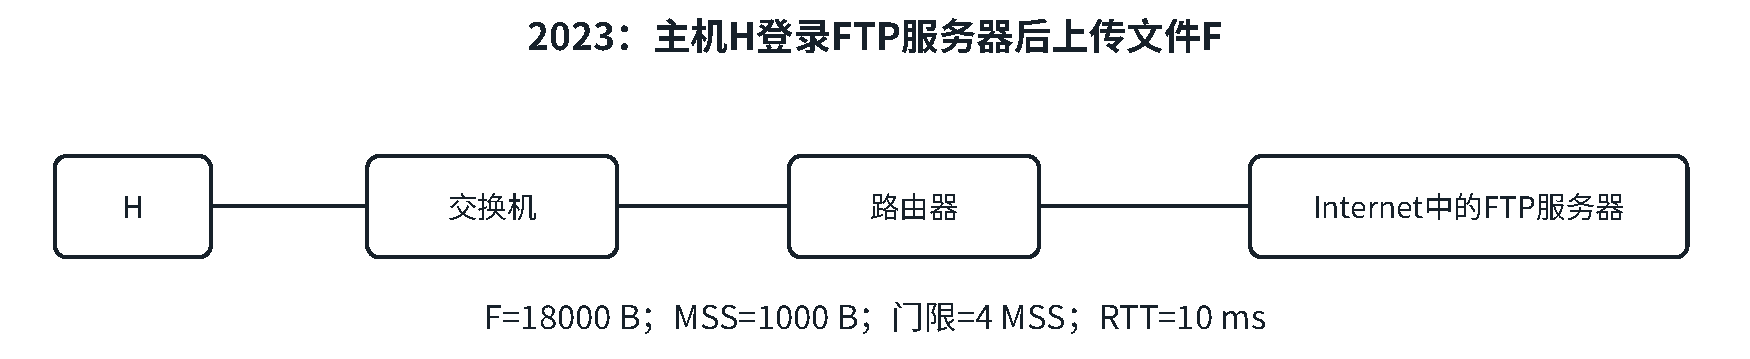
\includegraphics[width=\linewidth,height=125mm,keepaspectratio]{figures/CN26_ftp_2023.pdf}
\captionof{figure}{H经交换机、路由器访问Internet中的FTP服务器，控制连接与数据连接均由TCP承载}\label{cn-fig-ftp2023}
\end{minipage}\par\medskip

（1）FTP控制连接是持久的还是非持久的？数据连接是持久的还是非持久的？H登录服务器时建立的TCP连接是控制连接还是数据连接？

（2）H通过数据连接发送F时，F第1个字节的序号是多少？断开数据连接过程中，FTP服务器发送的第二次挥手ACK段的确认号是多少？

（3）当H收到确认号2101的确认段时，拥塞窗口调整为多少？收到确认号7101的确认段时，拥塞窗口调整为多少？

（4）H从请求建立数据连接开始，到确认F已被服务器全部接收，至少需要多久？期间应用层数据的平均发送速率是多少？

\end{example}

\textbf{解析。} 先把FTP会话与一次文件传输分开。控制连接在整个FTP会话期间保持，承载登录、命令与控制信息，因此是\textbf{持久连接}；本题的数据连接服务于本次文件传输，传完后关闭，是\textbf{非持久连接}。登录时先建立的是\textbf{控制连接}，已经完成的登录过程不再计入第（4）问的数据连接计时。

数据连接的SYN占序号100，F首字节从\textbf{101}开始。18000 B文件占序号101～18100，发送完后H的FIN占18101，服务器第二次挥手的ACK应确认下一个期望序号，故为\textbf{18102}。这里确认的是文件数据再加FIN，不能把登录控制连接的序号混进来。

拥塞控制沿用教材的轮次模型：初始\(cwnd=1\) MSS，达到4 MSS门限后按每RTT增加1 MSS。先看ACK落在哪个时刻：确认号2101累计确认\(2101-101=2000\) B，即前2个段。第1个ACK使cwnd从1增为2 MSS；第2个ACK是第二轮中较早的那个，此时仍在慢开始，cwnd从2增为\textbf{3 MSS}。不能把``第二轮结束时4 MSS''提前用于这个ACK。

确认号7101累计确认\(7101-101=7000\) B，即\(1+2+4=7\)个段，恰好完成第3轮。此轮开始时已到4 MSS门限，采用拥塞避免，第3轮结束后窗口为\textbf{5 MSS}。下表同时列出数据发送、确认时刻与累计量，时间均从数据连接SYN发出算起。

\begin{wideblock}

\par\medskip\noindent\begin{minipage}{\linewidth}\fontsize{9.3}{12}\selectfont\begin{tabularx}{\linewidth}{@{}YYYY@{}}
\toprule\noalign{}
阶段 & 开始时刻/ms & 本轮cwnd/MSS & 本轮发送段数 \\
\midrule\noalign{}


数据连接握手 & 0 & --- & --- \\
数据第1轮 & 10 & 1 & 1 \\
数据第2轮 & 20 & 2 & 2 \\
数据第3轮 & 30 & 4 & 4 \\
数据第4轮 & 40 & 5 & 5 \\
数据第5轮 & 50 & 6 & 6 \\
\bottomrule\end{tabularx}
\end{minipage}\par\medskip

\end{wideblock}

\begin{wideblock}

\par\medskip\noindent\begin{minipage}{\linewidth}\fontsize{9.3}{12}\selectfont\begin{tabularx}{\linewidth}{@{}YYY@{}}
\toprule\noalign{}
阶段 & 累计发送段数 & 本轮全部确认到达/ms \\
\midrule\noalign{}


数据连接握手 & 0 & 10 \\
数据第1轮 & 1 & 20 \\
数据第2轮 & 3 & 30 \\
数据第3轮 & 7 & 40 \\
数据第4轮 & 12 & 50 \\
数据第5轮 & 18 & 60 \\
\bottomrule\end{tabularx}
\end{minipage}\par\medskip

\end{wideblock}

建立数据连接用1 RTT，18个段按1、2、4、5、6分5轮发完，并在最后一轮结束时得到全文件确认，所以总计\(6\mathrm{RTT}=\mathbf{60\ ms}\)。期间应用层平均速率为\(18000\times8/0.060=\mathbf{2.4\ Mb/s}\)，也就是300000 B/s=0.3 MB/s。分母按题目包含握手、不包含连接释放；不能只用50 ms的数据传输阶段，也不能因服务器较早收到最后一比特就省去最后确认的回程。

这里的按轮增长是题目采用的教材近似，阈值前逐ACK检查仍有意义；拥塞避免阶段不宜把轮次表误解成每个ACK都使cwnd增加整整1 MSS。若要描述某个操作系统的精确逐ACK轨迹，还需其拥塞算法和ACK策略。

\subsection{例 6-9　从DNS到HTTP，交换机只学习实际发送者}\label{CN06-ex9}

\begin{example}[配套例题]

配套例题。 某网络拓扑如下图，以太网交换机S通过路由器R与Internet互联。路由器接口、本地DNS、H1、H2的IP地址与MAC地址如图。\(t_0\)时H1的ARP表和S的交换表均为空；H1此时用浏览器通过域名www.abc.com请求访问Web服务器。\(t_1>t_0\)时，S第一次收到封装HTTP请求报文的以太网帧。其间没有与此次Web访问无关的网络通信。

\par\medskip\noindent\begin{minipage}{\linewidth}
\centering
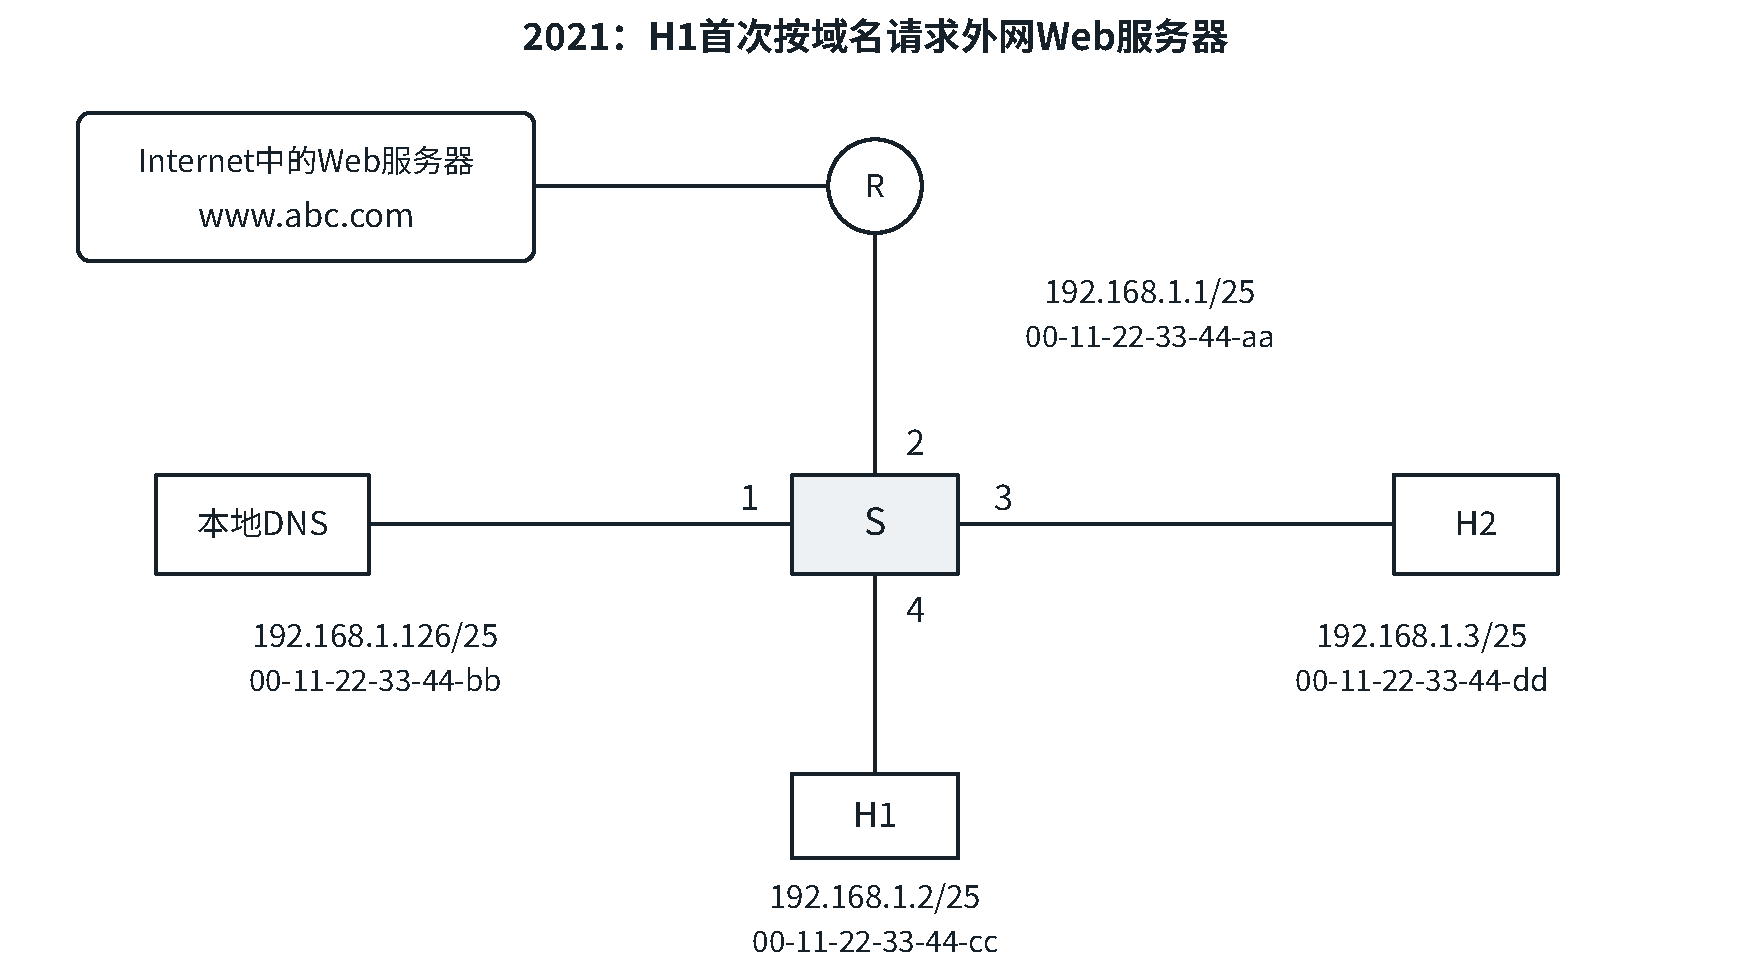
\includegraphics[width=\linewidth,height=125mm,keepaspectratio]{figures/CN27_dns_switch_2021.pdf}
\captionof{figure}{本地DNS接S的1口，R接2口，H2接3口，H1接4口；四者同属192.168.1.0/25}\label{cn-fig-dns-switch2021}
\end{minipage}\par\medskip

（1）从\(t_0\)到\(t_1\)，H1除HTTP外还运行哪个应用层协议？从应用层到数据链路层，该协议报文经过哪些协议逐层封装？

（2）S交换表结构为``MAC地址、端口''，\(t_1\)时交换表内容是什么？

（3）其间H2至少接收多少个与此次Web访问有关的帧？是什么帧？目的MAC地址是什么？

\end{example}

\textbf{解析。} 解题入口是按依赖关系列出``先知道谁的地址，才能发下一帧''。按本题及教材需要新做域名解析的流程，H1先运行\textbf{DNS}，把域名换成Web服务器IP；常规查询的封装为\textbf{DNS报文\ensuremath{\to}UDP数据报\ensuremath{\to}IPv4分组\ensuremath{\to}Ethernet II帧}。ARP用于在本地链路上解析MAC，不是DNS外面的一层，也不是另一个应用层协议；CSMA/CD是介质访问算法，不是帧格式，在全双工交换链路中通常不运行。

H1先根据\texttt{/\allowbreak{}25}判断本地DNS的192.168.1.126与自己同属192.168.1.0/25，先用ARP解析本地DNS的MAC地址，不先问网关。解析出Web服务器位于外网后，才ARP查询网关R的192.168.1.1。后续IP分组的最终目的仍是Web服务器，当前以太网帧的目的MAC却是R的MAC。

\begin{wideblock}

\par\medskip\noindent\begin{minipage}{\linewidth}\fontsize{9.3}{12}\selectfont\begin{tabularx}{\linewidth}{@{}YYYY@{}}
\toprule\noalign{}
\begin{minipage}[b]{\linewidth}\raggedright
顺序
\end{minipage} & \begin{minipage}[b]{\linewidth}\raggedright
S收到的帧
\end{minipage} & \begin{minipage}[b]{\linewidth}\raggedleft
入端口
\end{minipage} & \begin{minipage}[b]{\linewidth}\raggedright
S的处理与新增学习
\end{minipage} \\
\midrule\noalign{}


1 & H1广播ARP，询问本地DNS的MAC & 4 & 学习H1的cc\ensuremath{\to}4；向1、2、3口泛洪 \\
2 & DNS单播ARP应答给H1 & 1 & 学习DNS的bb\ensuremath{\to}1；已知cc，只转4口 \\
3 & H1单播DNS查询给DNS & 4 & 已知bb，只转1口 \\
4 & DNS单播查询应答给H1 & 1 & 已知cc，只转4口 \\
5 & H1广播ARP，询问网关R的MAC & 4 & 向1、2、3口泛洪 \\
6 & R单播ARP应答给H1 & 2 & 学习R的aa\ensuremath{\to}2；只转4口 \\
7 & H1向外网服务器发送TCP SYN，帧发给R & 4 & 已知aa，只转2口 \\
8 & R转发服务器的SYN+ACK，帧发给H1 & 2 & 已知cc，只转4口 \\
9 & H1发送TCP确认及首个HTTP请求 & 4 & 帧均发给R，只转2口；到达题设\(t_1\) \\
\bottomrule\end{tabularx}
\end{minipage}\par\medskip

\end{wideblock}

表中cc、bb、aa分别是下表完整MAC地址的末字节缩写。第三次握手ACK是否与首个HTTP请求合并，不改变学习或H2收到的帧数。交换机按\textbf{帧的源MAC与入端口}学习，不会从广播帧的目的地址、ARP询问目标、IP目的地址或题图上``知道有H2''便自行添加表项。因此\(t_1\)时为：

\begin{wideblock}

\par\medskip\noindent\begin{minipage}{\linewidth}\fontsize{9.3}{12}\selectfont\begin{tabularx}{\linewidth}{@{}YY@{}}
\toprule\noalign{}
MAC地址 & 端口 \\
\midrule\noalign{}


00-11-22-33-44-cc（H1） & 4 \\
00-11-22-33-44-bb（本地DNS） & 1 \\
00-11-22-33-44-aa（R） & 2 \\
\bottomrule\end{tabularx}
\end{minipage}\par\medskip

\end{wideblock}

H2只被动收到两次广播ARP请求，没有发出自己的帧，故没有dd\ensuremath{\to}3条目。两次单播应答到来时，交换机早已从相应请求学到H1的位置，不会因初始表为空便把所有单播一直泛洪。第（3）问按上述解析流程，H2至少收到\textbf{2个ARP请求帧}，分别查询本地DNS和网关，目的MAC均为\textbf{FF-FF-FF-FF-FF-FF}。

这个2帧结论以本题意图中的新DNS查询为前提。原题明确为空的是ARP表和交换表，并未额外声明DNS缓存为空；若允许命中已有DNS缓存，就不必先访问本地DNS，相应学习表与最小广播数都会改变。应保留这一条件边界，不能把``通过域名访问''推广成任何情况下都必然重新发送DNS查询。

\section{主动回忆自测}\label{CN06-review}

以下为自拟题。时间题先画依赖链，协议题先说谁向谁执行什么动作。

\begin{enumerate}
\def\labelenumi{\arabic{enumi}.}
\tightlist
\item
  HTML引用4个同站小图片，DNS已完成、TCP未建立，忽略发送和其他开销。持久非流水与持久流水各需多少RTT？
\item
  本地DNS已有目标域权威服务器地址、没有目标主机地址；到权威服务器RTT20 ms，TCP建立和HTTP请求响应各30 ms。局域网开销忽略，取纯文本页面至少多久？
\item
  收到304响应，能否说明本次完全没有网络往返？
\item
  C/S中的``客户''是否等于性能较低的机器？P2P使用集中索引后是否就只能由中心转发全部文件数据？
\item
  域与区为什么不必相同？A、AAAA、NS、MX各表达什么？
\item
  一次FTP登录与后续文件上传分别用哪类连接？所有FTP服务器数据端口都固定20吗？
\item
  SMTP、POP3与MIME分别做什么？Base64编码是否提供保密性？
\item
  URL中的片段\texttt{\#part1}是否通常随HTTP请求目标发给服务器？HTTP无状态能否推出不能使用持久TCP连接？
\item
  在新做DNS解析、ARP表和交换表为空的局域网访问流程中，交换机从目的MAC还是源MAC学习端口？DNS缓存命中会改变哪些步骤？
\end{enumerate}

\subsection{核对答案}\label{CN06-review-answers}

\begin{enumerate}
\def\labelenumi{\arabic{enumi}.}
\tightlist
\item
  非流水\(1+1+4=6\) RTT，流水\(1+1+1=3\) RTT；两者均包括首次TCP握手。
\item
  DNS20 ms，加Web两次30 ms，共80 ms；无需重新查询根与顶级服务器。
\item
  不能，304是网络条件验证响应，只省略完整实体传输。
\item
  客户是主动请求服务的角色；集中索引可以只协助发现，文件数据仍可在对等节点之间传输。
\item
  子域委派会让名称子树分属不同权威管理范围；四种记录分别指IPv4地址、IPv6地址、权威服务器和邮件交换。
\item
  登录命令走控制连接，文件走数据连接；被动模式的数据监听端口由服务器另行通告，不能一律固定20。
\item
  SMTP提交/转送、POP3读取、MIME描述内容类型与编码；Base64可公开解码，不是加密。
\item
  片段留在浏览器侧；无状态与连接复用是不同层次的问题，可以使用持久连接。
\item
  从源MAC与入端口学习；DNS缓存命中可能免去本次DNS查询以及为DNS服务端进行的ARP，对应交换表和广播计数也可能变化。
\end{enumerate}
